\documentclass{mwart}

            % Papier
\usepackage{polski}
\usepackage[utf8]{inputenc}
\usepackage[a4paper, total={16cm, 24cm}]{geometry}

            % Matematyka
\usepackage{amsthm}
\usepackage{amsmath}
\usepackage{amssymb}

           % Wygląd
%\usepackage{url}
\usepackage{hyperref}
\usepackage{graphics}
\usepackage{fancyhdr}
\usepackage{geometry}
\usepackage{enumitem}

            % Obrazki
\usepackage{graphicx}



            % Ustawienia ramek
\usepackage[nobreak=false]{mdframed}
\mdfsetup{%
% frametitlerule=true,
% subtitlebelowline=true,
subtitleaboveline=true,
subtitleaboveskip=0,
subtitlebelowskip=0,
linewidth=1pt}


% Skroty
\newcommand{\R}{\mathbb{R}}
\newcommand{\N}{\mathbb{N}}
\newcommand{\Z}{\mathbb{Z}}
\newcommand{\C}{\mathbb{C}}

\newtheorem{zad}{Zadanie}[section]

%Zmiana formatu sekcji
\renewcommand{\thesection}{\arabic{section}}


% Początek strony tytułowej


\author{\textbf{Grupa 3} \\ \textsf{Informatyka i Systemy Informacyjne | MiNI PW}}
\title{%
%\includegraphics[width=1\textwidth]{logo_uczelni.png}
\textbf{Matematyka Dyskretna I}}


%\setcounter{secnumdepth}{1}
\pagestyle{fancy}
\setlength{\headsep}{1.2cm}
\fancyhead{}
\lhead{Grupa 3\\\textsf{Wydział MiNI PW}}
\chead{\Large \textbf{Rozwiązania zadań}}
\rhead{\textbf{Matematyka Dyskretna 1}\\Informatyka}

\fancyfoot{}
\rfoot{\texttt{\thepage}}

\fancypagestyle{specialfooter}{%
    \fancyhf{}
    \renewcommand\headrulewidth{0pt}
    \fancyfoot[C]{\Large{Lato 2025}}
}


\begin{document}
\maketitle{}
\begin{center}
    Studenckie rozwiązania zadań z ćwiczeń z Matematyki Dyskretnej I. \\
    Ćwiczenia z \emph{MD I} w gr. 3 prowadzi dr inż. Tomasz Brengos \\
    i też oto pod jego opieką powstaje ten plik. \\
    Ostatnia aktualizacja: \today{} \\
    \tableofcontents
    \thispagestyle{specialfooter}

\end{center}

% Koniec strony tytułowej

















% Poczatek dokumentu
\newpage
\section{Zestaw}              % Zestaw 1
\begin{zad}[Krzysztof Wójtowicz, Autor 2]
    Na płaszczyźnie poprowadzono $n$ prostych, z których żadne dwie nie
    są równoległe i żadne trzy nie przechodzą przez ten sam punkt.
    Wyznacz liczbę:
    \begin{enumerate}
        \item obszarów, na które te proste dzielą płaszczyznę;
        \item obszarów ograniczonych, na które te proste dzielą płaszczyznę.
    \end{enumerate}
\end{zad}
\begin{mdframed}
    \begin{enumerate}
        % Rozwiązanie: Krzysztof Wójtowicz
        \item Zauważymy, że każda kolejna prosta przecina wszystkie poprzednie proste, 
        a co za tym idzie również obszary, które są do nich "przyległe", dzieląc je na 
        dwa. Każda poprzednia prosta ma dwa takie obszary, więc ich ogólna liczba to 
        (odejmujemy obszary wspólne, czyli te "pośrodku" dwóch prostych, by ich nie duplikować): 
        \[2(n-1) - (n-1-1) = n\] Zatem każda kolejna prosta dodaje n nowych obszarów: 
        \[P(n) = P(n-1) + n = P(0) + \sum_{k=1}^{n} k = 1 + \frac{n(n+1)}{2}\]
        gdzie $P(n)$ to liczba obszarów dla n prostych.
        \newline
        \item Liczbę obszarów ograniczonych otrzymamy odejmując liczbę obszarów nieograniczonych z wyniku z podpunku 1.
        Każda prosta ma dwa "przyległe" obszary nieograniczone, więc liczba wszystkich takich obszarów to $2n$,
        zatem liczba wszystkich obszarów ograniczonych to:
        \[1 + \frac{n(n+1)}{2} - 2n = \frac{n^2 - 3n + 2}{2} = \frac{(n-1)(n-2)}{2}\]
    \end{enumerate}
\end{mdframed}
\begin{mdframed}
    \begin{enumerate}
        \item Rozwiązanie Autora 2 podpunktu 1
        \item Rozwiązanie Autora 2 podpunktu 2
    \end{enumerate}
\end{mdframed}



\begin{zad}[Autor 1, Autor 2]
    Ciąg Fibonacciego $\{F_n\}_{n \in \mathbb{N}}$ zadany jest przez
    $F_0=0$, $F_1=1$ i $F_{n+2}=F_{n+1}+F_n$. Udowodnij, że: \\
    \begin{enumerate}
        \item $F_0 + ... + F_n = F_{n+2} - 1$;
        \item $5|F_{5n}$,
        \item $F_n < 2_n$.
    \end{enumerate}
\end{zad}
\begin{mdframed}
    \begin{enumerate}
        \item Rozwiązanie Autora 1 podpunktu 1
        \item Rozwiązanie Autora 1 podpunktu 2
        \item Rozwiązanie Autora 1 podpunktu 3
    \end{enumerate}
\end{mdframed}
\begin{mdframed}
    \begin{enumerate}
        \item Rozwiązanie Autora 2 podpunktu 1
        \item Rozwiązanie Autora 2 podpunktu 2
        \item Rozwiązanie Autora 2 podpunktu 3
    \end{enumerate}
\end{mdframed}




\begin{zad}[Autor 1, Autor 2]
    Turniej $n$-wierzchołkowy to dowolny graf skierowany $G = (V, E)$, gdzie $|V| = n$
    i w którym $(u, v) \in E$ lub $(v, u) \in E$ dla dowolnych $u, v \in V$.
    Pokaż, że w dowolnym niepustym turnieju istnieje wierzchołek z którego można “przejść”
    po krawędziach zgodnie z ich skierowaniem do dowolnego innego wierzchołka w co
    najwyżej dwóch krokach.
\end{zad}
\begin{mdframed}
    Rozwiązanie Autora 1.
\end{mdframed}
\begin{mdframed}
    Rozwiązanie Autora 2.
\end{mdframed}

\begin{zad}[Autor 1, Autor 2]
    Udowodnij, że każdy turniej ma ścieżkę Hamiltona.
\end{zad}
\begin{mdframed}
    Rozwiązanie Autora 1.
\end{mdframed}
\begin{mdframed}
    Rozwiązanie Autora 2.
\end{mdframed}




\begin{zad}[Autor 1, Autor 2]
    W każdym polu szachownicy rozmiaru $n x n $ znajduje się jedna osoba.
    Część osób zarażona jest wirusem grypy. Wirus grypy rozprzestrzenia się w dyskretnych
    odstępach czasowych w sposób następujący:
    \begin{itemize}
        \item osoby zarażone pozostają zarażone,
        \item osoba ulega zarażeniu jeżeli co najmniej dwie sąsiadujące z nią osoby są już zarażone
              (przez osobę sąsiednią rozumiemy osobę siedzącą z przodu, z tyłu, z lewej lub prawej
              strony).
              Wykaż, że jeżeli na początku zarażonych jest istotnie mniej niż n osób, to w każdej chwili
              przynajmniej jedna osoba pozostaje niezarażona.
    \end{itemize}
\end{zad}
\begin{mdframed}
    Rozwiązanie Autora 1.
\end{mdframed}
\begin{mdframed}
    Rozwiązanie Autora 2.
\end{mdframed}




\begin{zad}[Krzysztof Wójtowicz, Autor 2]
    Wykaż, że w grupie $n$ osób istnieją dwie, które mają taką samą liczbę znajomych.
\end{zad}
\begin{mdframed}
    \underline{Dowód:}
    \newline
    W grupie $n$ osób każda osoba może mieć od $0$ do $n-1$ znajomych, ale wtedy:
    \begin{enumerate}
    \item Jeśli ktoś ma $0$ znajomych to maksymalna liczba znajomych to $n-2$, bo osoba mająca $n-1$ znajomych
    musiałaby być znajomym z osobą, która ma ich $0$, co jest niemożliwe
    \item Jeśli minimalna liczba znajomych to $1$ to wtedy maksymalna liczba znajomych to $n-1$
    \end{enumerate}
    W obydwu przypadkach mamy $n-1$ wartości oraz $n$ osób. Zatem na mocy zasady Dirichleta conajmniej dwie
    osoby muszą mieć tę samą liczbę znajomych. 
    $\blacksquare$
\end{mdframed}
\begin{mdframed}
    Rozwiązanie Autora 2.
\end{mdframed}




\begin{zad}[Autor 1, Autor 2]
    Przy okrągłym stole jest $n$ miejsc oznaczonych proporczykami różnych
    państw. Ambasadorowie tych państw usiedli przy tym stole tak, że żaden z nich nie siadł
    przy właściwym proporczyku. Wykaż, że można tak obrócić stołem, że co najmniej 2
    ambasadorów znajdzie się przed proporczykiem swojego państwa.
\end{zad}
\begin{mdframed}
    Rozwiązanie Autora 1.
\end{mdframed}
\begin{mdframed}
    Rozwiązanie Autora 2.
\end{mdframed}




\begin{zad}[Autor 1, Autor 2]
    Pokaż, że w dowolnym ciągu n liczb całkowitych istnieje (niepusty)
    podciąg kolejnych elementów taki, że suma wyrazów podciągu jest wielokrotnością n.
\end{zad}
\begin{mdframed}
    Rozwiązanie Autora 1.
\end{mdframed}
\begin{mdframed}
    Rozwiązanie Autora 2.
\end{mdframed}




\begin{zad}[Autor 1, Autor 2]
    Rozważ dowolną rodzinę podzbiorów zbioru $n$--elementowego zawierającą
    więcej niż połowę wszystkich podzbiorów. Wykaż, że w tej rodzinie muszą być dwa zbiory
    takie, że jeden zawiera się w drugim.
\end{zad}
\begin{mdframed}
    Rozwiązanie Autora 1.
\end{mdframed}
\begin{mdframed}
    Rozwiązanie Autora 2.
\end{mdframed}



\begin{zad}[Autor 1, Autor 2]
    Dla $n$--elementowego zbioru $X$ rozważ pewną rodzinę jego podzbiorów
    $\mathcal{F}$, gdzie $|F| > n/2$ dla każdego $F \in \mathcal{F}$. Wykaż, że istnieje
    $x \in X$ należący do co najmniej połowy zbiorów z $\mathcal{F}$.
\end{zad}
\begin{mdframed}
    Rozwiązanie Autora 1.
\end{mdframed}
\begin{mdframed}
    Rozwiązanie Autora 2.
\end{mdframed}


\begin{zad}[Autor 1, Autor 2]
    Dana jest kwadratowa szachownica $n \times n$. Dla jakich wartosci $n\geq 1$
    możemy pokryć tę szachownicę kostkami wielkości $2 \times 2$ oraz $3 \times 3$.
\end{zad}
\begin{mdframed}
    Rozwiązanie Autora 1.
\end{mdframed}
\begin{mdframed}
    Rozwiązanie Autora 2.
\end{mdframed}


\begin{zad}[Autor 1, Autor 2]
    Dana jest kwadratowa szachownica $2n \times 2n$ z wyciętym jednym polem.
    Wykaż, że dla wszystkich wartości $n \geq 1$ możemy pokryć tę szachownicę kostkami w
    kształcie litery L (czyli kwadrat $2 \times 2$ bez jednego pola).
\end{zad}
\begin{mdframed}
    Rozwiązanie Autora 1.
\end{mdframed}
\begin{mdframed}
    Rozwiązanie Autora 2.
\end{mdframed}






















\newpage
\section{Zestaw}          % ZESTAW 2

\begin{zad}[Filip Sajko, Bartłomiej Sokołowski]
    Na ile sposobów można ustawić $n$ wież na szachownicy
    $n \times n$ tak, by żadne dwie nie znajdowały się w
    polu wzajemnego rażenia.
\end{zad}
\begin{mdframed}
    Starczy zauważyć, że dla każdej wieży wybieramy rząd i kolumnę
    w której się znajduje -- i tym samym zmniejsza liczbę dostępnych
    o jeden. Tak więc odpowiedź wynosi: \[n \cdot n \cdot (n-1) \cdot
        (n-1) \cdot ... \cdot 2 \cdot 2 \cdot 1 \cdot 1 =  n! \cdot n!\]
\end{mdframed}
\begin{mdframed}
    %Rozwiązanie: Bartłomiej Sokołowski
    Musimy wybrać $n$ pozycji z $n^2$ dostępnych pól na szachownicy. Wybierając 
    $1$ pozycję automatycznie eliminujemy całą kolumnę oraz wiersz, w którym znajduje się wybrane pole.
    \item Pierwszą wieżę wybieramy z $n \times n = n^2$ dostępnych pozycji.
    \item Następną wieżę wybieramy na $(n-1) \times (n-1) = (n-1)^2$ sposobów, ponieważ wykluczamy wybraną już kolumnę i wiersz.
    \item Powtarzając proces $n$ razy dostajemy:
    \[n \times n \times (n-1) \times (n - 1) \times ... \times 1 \times 1 = n! \times n! = (n!)^2\] 
\end{mdframed}




\begin{zad}[Filip Sajko, Autor 2]
    Na ile sposobów można ustawić $k$ wież na szachownicy $n \times m$
    tak, by żadne dwie nie znajdowały się w polu wzajemnego rażenia.
\end{zad}
\begin{mdframed}
    Zadanie analogiczne od poprzedniego - z tym, że zmienił nam się
    rozmiar planszy, a ponadto nie wypełniamy jej całej. Zasada
    pozostaje jednak ta sama. Na start jednak warto założyć, że
    $k \leq max\{n, m\}$ (choć w sumie jeżeli tak nie jest, to
    odpowiedź to 0). Mając to już za sobą:
    \[n \cdot m \cdot (n-1) \cdot (m-1) \cdot ... \cdot (n - k +1) \cdot (m -k +1)\]
    (wykonujemy mnożenie $k + k$ elementów -- stąd to $-k + 1$).
\end{mdframed}
\begin{mdframed}
    Rozwiązanie Autora 2.
\end{mdframed}




\begin{zad}[Filip Sajko, Autor 2]
    Znaleźć definicje rekurencyjne następujących ciągów:
    \begin{enumerate}
        \item $a(n)$ -- liczba słów długości $n$ nad alfabetem
              $\{0, 1\}$, które nie zawierają dwóch jedynek koło siebie.
        \item  $b(n)$ -- liczba różnych pokryć prostokąta o wymiarze
              $2 \times n$ dominami wymiaru $2 \times 1$.
    \end{enumerate}
\end{zad}
\begin{mdframed}
    \begin{enumerate}

        \item Oczywiście $a(1)=2$, $a(2)=3$.  Rozważmy słowo $n$ elementowe.
              Zauważamy, że jeżeli ono kończy sie ono zerem to poprzedzające słowo $n-1$
              elementowe jest dowolne. Jeżeli natomiast kończy się jedynką,
              to poprzedzające słowo $n-2$ elementowe jest dowolne
              (tak jakby cofamy się krok dalej by mieć dowolność).
              Stąd: $a(n)=a(n-1)+a(n-2)$.
        \item Analogicznie do poprzedniego. Jak wiemy $a(1) = 1$, $a(2) = 2$. Zastanówmy się nad $a(n)$:
              Rozważamy ciąg o długości $n$. Jeżeli na końcu jest blok poziomy,
              to wiemy że powstał on z ciągu długości $a(n-2)$.
              Jeżeli jest pionowy, to wiemy, że musiał on powstać z ciągu długości $n-1$.
              A stąd $a(n) = a(n-1) + a(n-2)$.
    \end{enumerate}
\end{mdframed}
\begin{mdframed}
    Rozwiązanie Autora 2.
\end{mdframed}




\begin{zad}[Autor 1, Autor 2]
    Ile rozwiązań ma równanie $x_1 + x_2+x_3+x_4 = 7$:
    \begin{enumerate}
        \item gdzie $x_i$ są liczbami naturalnymi?
        \item gdzie $x_i$ są dodatnimi liczbami naturalnymi?
    \end{enumerate}
\end{zad}
\begin{mdframed}
    \begin{enumerate}
        \item Rozwiązanie Autora 1 podpunktu 1
        \item Rozwiązanie Autora 1 podpunktu 2
    \end{enumerate}
\end{mdframed}
\begin{mdframed}
    \begin{enumerate}
        \item Rozwiązanie Autora 2 podpunktu 1
        \item Rozwiązanie Autora 2 podpunktu 2
    \end{enumerate}
\end{mdframed}




\begin{zad}[Autor 1, Autor 2]
    Rozważmy czekoladę złożoną z $m\times n$ kostek.
    Na ile sposobów można wykroić prostokąt złożony z $k \times k$
    sąsiadujących ze sobą kostek czekolady?
\end{zad}
\begin{mdframed}
    Rozwiązanie Autora 1.
\end{mdframed}
\begin{mdframed}
    Rozwiązanie Autora 2.
\end{mdframed}




\begin{zad}[Maciej Wełpa, Autor 2]
    (Reguła sumowania po górnym indeksie). Udowodnij, że dla
    $n, k \in \mathbb{N}$ zachodzi
    \[\sum_{j=0}^n\binom{j}{k} = \binom{n+1}{k+1}\]
\end{zad}
\begin{mdframed}
    % Rozwiązanie: Maciej Wełpa
    \textbf{Lewa strona:} 
    Niech X to zbiór wszystkich k + 1 elementów z ze zbioru n + 1 elementów, \\
    \(|X|\) = \(\binom{n + 1}{k + 1}\). \\ 
    \textbf{Prawa strona:} Niech \( X_j \) to podzbiory \(|k+1|\) elementowe ze zbioru X, które
    zawierają maksymalny element j+1. np. dla k = 2 \( X_3 \) = \{1, 2, 4\}, \( X_4 \) = \{1, 3, 5\} 
    - ostatni element jest największy, pozostałe dwa to wybrane z \{1...j\}. Rozważamy j elementów mniejszych od j+1, spośród nich wybieramy k elementów - mamy \(\binom{j}{k}\) możliwości. Sumując po j dodajemy do siebie wszystkie możliwości.
\end{mdframed}
\begin{mdframed}
    Rozwiązanie Autora 2.
\end{mdframed}




\begin{zad}[Bartłomiej Sokołowski, Autor 2]
    (Reguła sumowania równoległego). Udowodnij, że dla $n, k \in \mathbb{N}$
    zachodzi \[ \sum_{j= 0}^{n}\binom{n+j}{j} = \binom{n+k+1}{k}   \]
\end{zad}\
\begin{mdframed}
    %Rozwiązanie: Bartłomiej Sokołowski 
    Przeprowadzimy dowód indukcyjny. 
    \item k = 0:
    \item \[ L = \sum_{j=0}^{0}\binom{n+j}{j} = \binom{n}{0} = 0 \] 
    \item \[P = \binom{n+0+1}{0} = \binom{n+1}{0} = 0\]
    \item Zał. indukcyjne :
    \item \[\sum_{j=0}^{k}\binom{n+j}{j} = \binom{n+k+1}{k}\]
    \item Teza indukcyjna :
    \item \[\sum_{j=0}^{k+1}\binom{n+j}{j} = \binom{n+k+2}{k+1}\]
    \item \[\sum_{j=0}^{k+1}\binom{n+j}{j} = \sum_{j=0}^{k}\binom{n+j}{j} + \binom{n+k+1}{k+1} = \binom{n+k+1}{k} + \binom{n+k+1}{k+1} = \binom{n+k+2}{k+1}\]
\end{mdframed}
\begin{mdframed}
    Rozwiązanie Autora 2.
\end{mdframed}



\begin{zad}[Krzysztof Wojczakowski, Autor 2]
    Ile jest funkcji $f:\{1, ..., n\} \to \{1, ..., n\}$ monotonicznych takich,
    że $f(i) \leq f(j) $ dla $i < j$?
\end{zad}
\begin{mdframed}
    %Rozwiązanie: Krzysztof Wojczakowski
    Zauważmy, że te funkcje tworza tak jakby jakby ciąg , który ma być niemalejący. 
    Możemy to zobrazować jako kratę gdzie wartości na dole to liczby od 1 do n , a idąc do góry 
    mozemy tylko iść w prawo lub w górę. , gdie tyle ile kresek w górę przy danej liczbie to tyle ile razy tą liczbę wybieramy.
    \vspace{0.3em} % mały odstęp w pionie

    \noindent
    \centering
    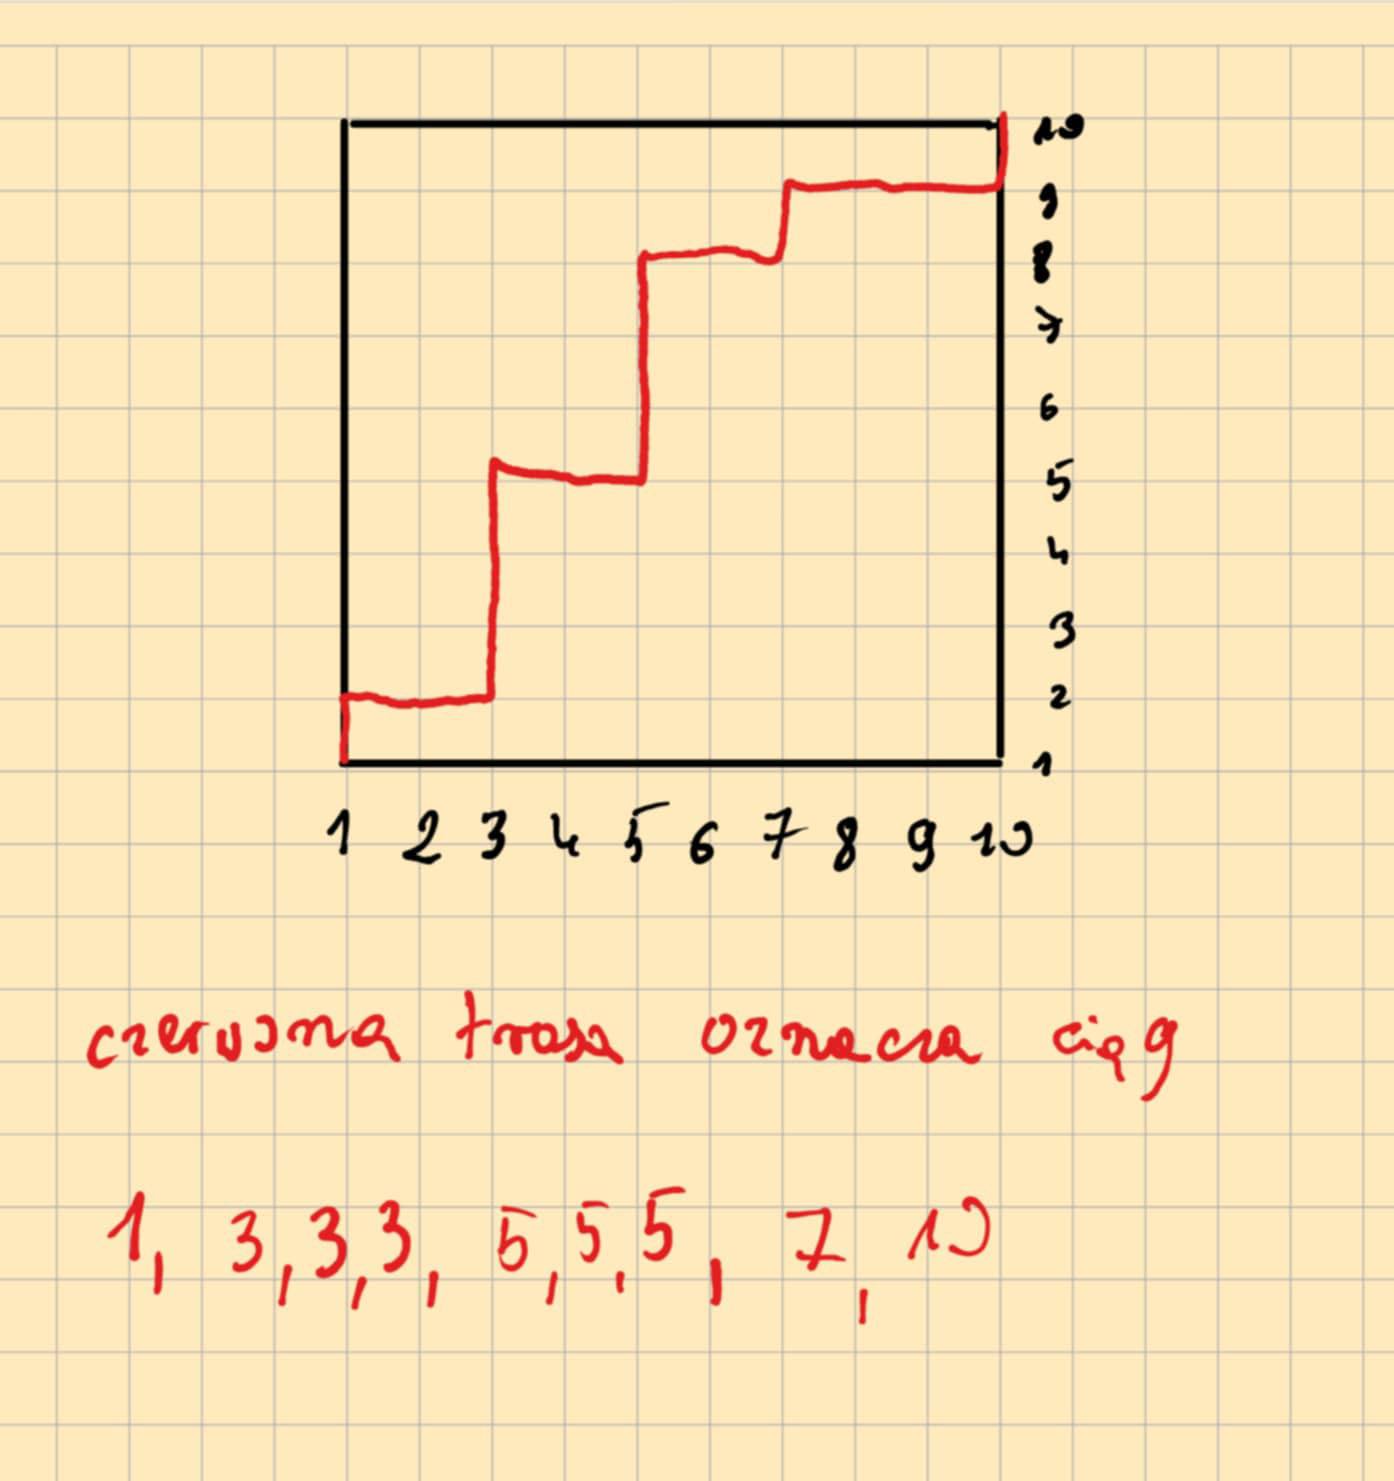
\includegraphics[width=0.7\textwidth]{images/zadanie28.png}

    Końcowo poszliśmy $n-1$ razy w prawo i $n-1$ razy w górę, czyli mamy $n-1+n-1 = 2n - 2$ kroków
    W rezultacie takich funkcji jest:
    \( \binom{2n-2}{n-1} \)
\end{mdframed}
\begin{mdframed}
    Rozwiązanie Autora 2.
\end{mdframed}




\begin{zad}[Krzysztof Wojczakowski, Autor 2]
    Ile jest $k$--elementowych podzbiorów zbioru $n$--elementowego, które nie
    zawierają dwóch sąsiednich liczb?
\end{zad}
\begin{mdframed}
    %Rozwiązanie: Krzysztof Wojczakowski
    Zauważmy, że jeżeli mamy mamy do wybrania $k$ elementow , to równolegle to oznacza , że 
    musimy zrobić $k-1$ "przerw" pomiędzy nimi. Wygląda to tak:
    \verb|_0_0_0_..._0_0_| 
    gdzie zero to oznacza ze liczby nie bierzemy, a podłoga oznacza, że bierzemy. 
    Zostaje nam $n-(k+1)$ miejsc do wyboru, czyli $n-k+1$ miejsc.
    w takim razie ilość $k$ elementowych podzbiorów jest : 
    \( \binom{n-k+1}{k} \)

\end{mdframed}
\begin{mdframed}
    Rozwiązanie Autora 2.
\end{mdframed}


\begin{zad}[Autor 1, Autor 2]
    Posługując się interpretacją kombinatoryczną udowodnij, że:
    \[ \sum_{i=0}^{k} \binom{n}{i} \binom{n-i}{k-i} = 2^k \binom{n}{k} \]
\end{zad}
\begin{mdframed}
    Rozwiązanie Autora 1.
\end{mdframed}
\begin{mdframed}
    Rozwiązanie Autora 2.
\end{mdframed}




\begin{zad}[Katarzyna Szwed, Autor 2]
    Udowodnij poniższe tożsamości na dwa sposoby: posługując się interpretacją
    kombinatoryczną albo rozwinięciem dwumianu $(1 + x)^n$:
    \begin{enumerate}
        \item \[\sum_{k=0}^{n}k\binom{n}{k} = n2^{n-1}\]
        \item \[\sum_{k=0}^{n}k^2\binom{n}{k}= (n+n^2)2^{n-2}\]
        \item \[\sum_{i=0}^{k}\binom{m}{i}\binom{n}{k-i} = \binom{m+n}{k} \]
    \end{enumerate}
\end{zad}
\begin{mdframed}
    %Rozwiązanie: Katarzyna Szwed
    \begin{enumerate}
        \item Podpunkt 1

        Rozważmy zbiór $X$ taki, że:
        \[X := \{ (A, x) : x \in A \wedge A \subset [n]\}\]

        Żeby policzyć jego moc najpierw wybierzemy element $x \in [n]$ na $n$ sposobów, 
        a potem resztę elementów zbioru $A$, czyli dowolny podzbiór $[n]-\{x\}$
        \[|X| = n \cdot 2^{n-1}\] 

        Teraz rozważmy rodzinę zbiorów $\{X_k\}_{k=0}^n$:
        \[X_k := \{(A, x) \in X : |A| = k\}\]

        Żeby policzyć moc zbioru $X_k$ (dla danego $k$) najpierw wybieramy $k$-elementowy zbiór $A$ będący podzbiorem $[n]$, a potem należący
        do niego element $x$:
        \[|X_k| = {n \choose k} \cdot k\]  

        Rodzina $X_k$ jest rozłącznym pokryciem zbioru $X$, zatem mamy:
        \[|X| = \sum_{k=0}^{n} |X_k|\]
        \[n \cdot 2^{n-1} = \sum_{k=0}^{n} k \cdot {n \choose k}\]

        \item Podpunkt 2

        Rozważmy zbiór $X$ taki, że:
        \[X := \{(A, x_1, x_2) : A \subset [n] \wedge x_1, x_2 \in A\}\]

        Żeby policzyć moc zbioru $X$ osobno policzymy przypadki kiedy $x_1 = x_2$ i $x_1 \neq x_2$.

        Dla $x_1 = x_2$ wybieramy najpierw wyróżniony element na $n$ sposobów, a potem dobieramy resztę elementów z $A$, 
        dostajemy $n2^{n-1}$.

        Dla $x_1 \neq x_2$ wybieramy $x_1$ na $n$ sposobów, $x_2$ na $n-1$ sposobów, a potem dobieramy resztę elementów z $A$, 
        dostajemy $n(n-1)2^{n-2}$. 
        Zatem mamy:
        \[|X| = n2^{n-1} + n(n-1)2^{n-2} = (2n + n^2 - n)2^{n-2} = (n + n^2)2^{n-2}\]

        Teraz rozważmy rodzinę zbiorów $\{X_k\}_{k=0}^n$:
        \[X_k := \{(A, x_1, x_2) \in X : |A| = k\}\]

        Żeby policzyć moc zbioru $X_k$ (dla danego $k$) najpierw wybierzemy $k$-elementowy zbiór $A \subset [n]$, a potem wybierzemy z niego elementy 
        $x_1$ i $x_2$ (przy czym mogą być one sobie równe):
        \[|X_k| = {n \choose k} \cdot k\cdot k\]

        Rodzina $X_k$ jest rozłącznym pokryciem zbioru $X$, więc otrzymujemy:
        \[\sum_{k=0}^{n} |X_k| = |X|\]
        \[\sum_{k=0}^{n}k^2{n \choose k}= n(n+1)2^{n-2}\]

        \item Podpunkt 3

        Rozważmy zbiór $X$ taki, że:
        \[X := \{A \subset [m + n] : |A| = k\}\]

        Zauważmy, że $|X| = {m+n \choose k}$.

        Teraz rozważmy rodzinę zbiorów $\{X_i\}_{i=0}^n$:
        \[X_i := \{A \in X : |A \cap [m]| = i\}\]
        
        Żeby policzyć moc zbioru $X_i$ (dla danego $i$) najpierw wybieramy $i$ elementów z $[m]$, a potem $k-i$ elementów z 
        $\{m+1, m+2, ..., m+n\}$, zatem $|X_i| = {m \choose i}{n \choose k-i}$.

        Rodzina $X_i$ jest rozłącznym pokryciem zbioru $X$, więc otrzymujemy:
        \[|X| = \sum_{i=0}^{n} |X_i|\]
        \[{m+n \choose k} = \sum_{i=0}^{k}{m \choose i}{n \choose k-i}\]

    \end{enumerate}
\end{mdframed}
\begin{mdframed}
    \begin{enumerate}
        \item Rozwiązanie Autora 2 podpunktu 1
        \item Rozwiązanie Autora 2 podpunktu 2
        \item Rozwiązanie Autora 2 podpunktu 3
    \end{enumerate}
\end{mdframed}






















\newpage
\section{Zestaw}          % ZESTAW 3

\begin{zad}[Autor 1, Autor 2]
    Wykaż, że dla dowolnego $n \geq 1$ istnieje $k \geq 1$ takie, że:
    \[S(n, 0) < S(n, 1) < ... < S(n, k - 1 ) \leq S(n, k) > S(n, k+1) > ... > S(n, n)\]
\end{zad}
\begin{mdframed}
    Rozwiązanie Autora 1.
\end{mdframed}
\begin{mdframed}
    Rozwiązanie Autora 2.
\end{mdframed}




\begin{zad}[Bartłomiej Sokołowski , Autor 2]
    Wykaż, że:
    \[B(n) = \sum_{i=0}^{n-1} \binom{n-1}{i}B(i)\]
\end{zad}
\begin{mdframed}
    %Rozwiązanie: Bartłomiej Sokołowski 
    \item Dowód:
    \item Niech $X = \pi([n])$, wtedy $|X| = B(n)$
    \item Niech $X_i = \{\pi([n]) : \exists_{A \in \pi([n])} (n \in A \land |A| = i + 1)\}$
    \item Jest to zbiór wszystkich podziałów, które zawierają n oraz mają wielkość i+1
    \item Jest to rozłączne pokrycie zbioru X 
    \item \[ |X_i| = \binom{n-1}{i} \times B(n-i-1)\]
    \item gdzie $\binom{n-1}{i}$ reprezentuje wybór $i$ elementów z bloku z $n$, a $B(n-i-1)$ reprezentuje podzielenie pozostałych elementów na bloki.
    \item \[ |X| = \sum_{i=0}^{n-1} |X_i| = \sum_{i=0}^{n-1}\binom{n-1}{i} \times B(n-i-1) = \sum_{i=0}^{n-1} \binom{n-1}{n-i-1} \times B(n-i-1) = \sum_{i=0}^{n-1} \binom{n-1}{i} \times B(i)\]
    \item Ostatnie przejście to sumowanie ale od drugiej strony, dlatego można je wykonać.
\end{mdframed}
\begin{mdframed}
    Rozwiązanie Autora 2.
\end{mdframed}




\begin{zad}[Autor 1, Autor 2]
    Wykaż, że dla $n, k \in \mathbb{N}$ zachodzi:
    \[S(n,k+1)=\frac{1}{(k+1)!} \sum_{0<i_0<...<i_{k-1}<n} \binom{n}{i_{k-1}}\binom{i_{k-1}}{i_{k_2}}...\binom{i_1}{i_0}     \]
\end{zad}
\begin{mdframed}
    Rozwiązanie Autora 1.
\end{mdframed}
\begin{mdframed}
    Rozwiązanie Autora 2.
\end{mdframed}





\begin{zad}[Autor 1, Autor 2]
    Rozważ  następującą procedurę generującą pewne liczby naturalne
    $\{a_{i,j}\}_{1 \geq i \geq j}$:
    \begin{enumerate}
        \item $a_{0,0} = 1$,
        \item $a_{n+1, 0} = a_{n,n}$, dla $n \geq 0$,
        \item $a_{n+1, k+1} = a_{n, k} + a_{n+1, k}$, dla $n \geq k \geq 0$.
    \end{enumerate}
\end{zad}
\begin{mdframed}
    Rozwiązanie Autora 1.
\end{mdframed}
\begin{mdframed}
    Rozwiązanie Autora 2.
\end{mdframed}




\begin{zad}[Bartosz Wójcik, Autor 2]
    Wykaż, że liczba podziałów zbioru $(n - 1)$  elementowego jest równa
    liczbie podziałów zbioru $\{1, ..., n\}$ niezawierających sąsiednich liczb w jednym bloku.
\end{zad}

\begin{mdframed}
    % Rozwiązanie: Bartosz Wójcik
    Niech $X$ będzie zbiorem podziałów zbioru $[n]$, takich że sąsiednie liczby nie 
    znajdują się w jednym bloku. Niech $Y$ będzie zbiorem podziałów zbioru $[n - 1]$. 
    Niech $ f : X \rightarrow Y$ będzie funkcją taką że jeśli $f(x) = y$:
    \begin{itemize}
        \item Dla każdego $i$, które należy do tego samego bloku co $n$ w zbiorze $x$ w zbiorze \
        $y$ istnieje blok $A$ taki że $i, i + 1 \in A$
        \item Jeśli $i$ należy do bloku $B$ w zbiorze $x$, który nie zawiera $n$ to istnieje blok \
        $B' \in y$, taki że $B \subseteq B'$
    \end{itemize}
    Przykładowo:
    
    $$\
    \{\{2, 4\}, \{1, 3\}\} \mapsto \{\{1, 2, 3\}\} \
    $$

    Funkcja $f$ jest dobrze zdefiniowana, ponieważ dla każdego $i$ jednoznacznie wyznaczony jest blok, 
    w którym się znajdzie - jeśli $i$ należało do bloku z $n$, to zostanie przerzucone do bloku z $i + 1$ 
    ($i + 1$ nie może się znajdować w tym samym bloku co $n$, ponieważ elementy nie sąsiadują). W przeciwnym 
    wypadku $i$ zostaje w tym bloku co było.

    Udowodnimy, że $f$ jest bijekcją. Niech $x_1, x_2 \in X$. Niech każdy blok $A_i$ będzie indeksowany najwyższym elementem 
    w danym bloku. Dla danego podziału $x$ indeksowanie bloków się nie zmienia (poza blokiem $A_n$, który znika), ponieważ 
    bloki po funkcji $f$ tylko zyskują elementy niższe niż najwyższy element. Załóżmy, że $x_1 \neq x_2$. Jeśli $x_1$ i $x_2$ 
    różnią sie na bloku $A_n$ (który zawsze należy do podziału) to $f(x_1)$ będzie miało różny zbiór elementów, które ze sobą sąsiadują.
    W przeciwnym wypadku istnieją $i_1$ oraz $i_2$, które w $x_1$ są w tym samym bloku, a w $x_2$ nie (lub na odwrót). Funkcja f nie 
    przestawia tych elementów, więc $f(x_1) \neq f(x_2)$.

    Rozważmy $y \in Y$. Znajdziemy $x \in X$, takie że $f(x) = y$. Rozważmy zbiór $S$ wszystkich elementów, które mają swojego sąsiada w tym 
    samym bloku w $y$. Skonstruujmy podział $x$ w następujący sposób:

    \begin{itemize}
        \item Utwórzmy nowy blok $A_n$, taki że $n \in A_n$
        \item Weźmy najmniejszy element z $S$ i dodajmy go do $A_n$. Proces powtórzmy dla kolejnego najmniejszego elementu w $S$, takiego że \
        ten element nie ma już swojego sąsiada w $A_n$. Procedura kończy się, kiedy skoonstruowany podział nie ma już elementów sąsiadujących.
    \end{itemize}

    Wtedy $f(x) = y$, więc $f$ jest bijekcją, co kończy dowód.

\end{mdframed}

\begin{mdframed}
    Rozwiązanie Autora 2.
\end{mdframed}




\begin{zad}[Maciej Wełpa, Autor 2]
    Udowodnij, że liczba ukorzenionych drzew binarnych na $n$ wierzchołkach to $n$-ta liczba Catalana.

    Ukorzenione drzewo jest drzewem binarnym, jeśli każdy wierzchołek ma co najwyżej
    dwójkę dzieci przy czym co najwyżej jedno lewe dziecko i co najwyżej jedno prawe dziecko.
\end{zad}
\begin{mdframed}
    % Rozwiązanie: Maciej Wełpa
    Spośród n wierzchołków, jeden wykorzystujemy na wierzchołek.\\
    Spośród pozostałych n-1 wybieramy i na lewe poddrzewo, a pozostałe n-1-i na prawe. W ten sposób możemy postępować rekurencyjnie\\
    Załóżmy funkcję \( T(k) \), która liczy ilość drzew. Jest ona rekurencyjna, bo każdy nowy korzeń może utworzyć nowe drzewo, a ilość korzeni lewo/prawo może się zmieniać, więc aby policzyć wszystkie możliwości skorzystamy z sumy.
    \[
    T(n) = \sum_{i=0}^{n-1} T(i) \cdot T(n-1-i)
    \]
    a to odpowiada rekurencyjnemu wzorowi Catalana.
    \begin{center}
    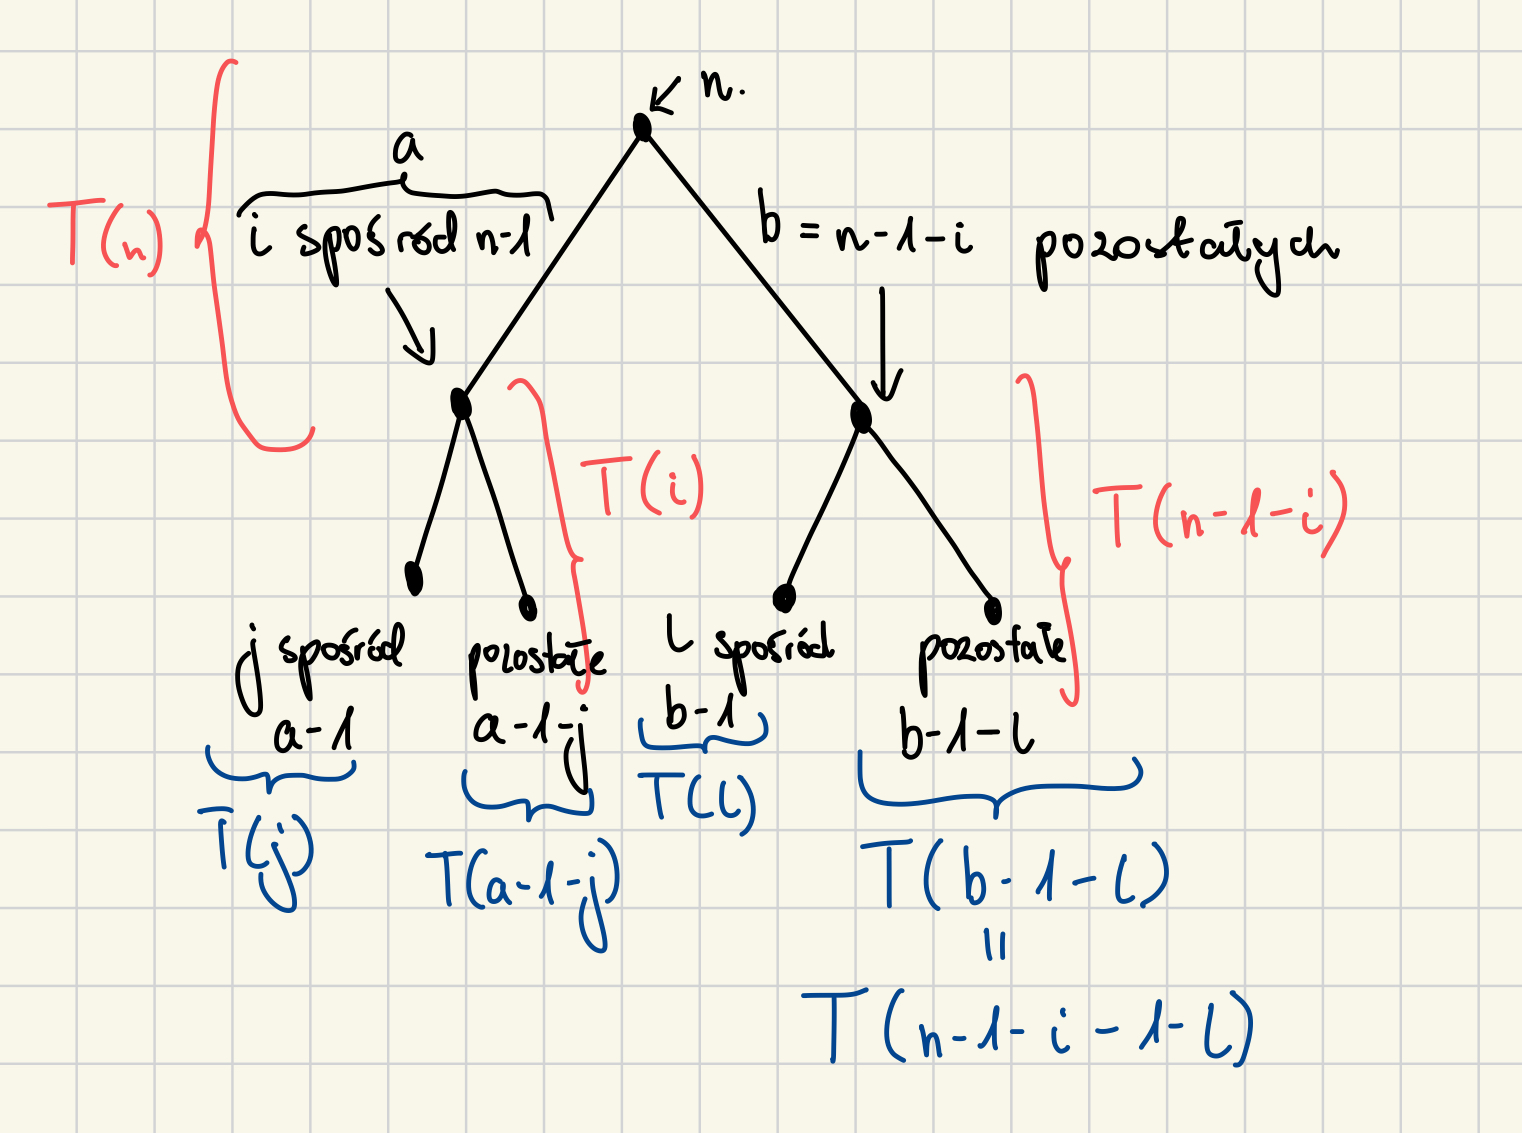
\includegraphics[width=0.7\textwidth]{images/zad36.jpeg}
\end{center}

\end{mdframed}
\begin{mdframed}
    Rozwiązanie Autora 2.
\end{mdframed}




\begin{zad}[Autor 1, Autor 2]
    Triangulacją $n$ -- wierzchołkowego wielokąta wypukłego nazywamy zbiór
    $(n - 3)$ wzajemnie nieprzecinających się jego przekątnych, które dzielą jego obszar na
    $(n - 2)$ trójkątów.
    \begin{enumerate}
        \item ile jest triangulacji $n$--wierzchołkowego wielokąta wypukłego?
        \item Ile jest triangulacji $n$--wierzchołkowego wielokąta wypukłego, w których każdy trójkąt
              triangulacji ma przynajmniej jeden bok na brzegu wielokąta?
    \end{enumerate}
\end{zad}
\begin{mdframed}
    \begin{enumerate}
        \item Rozwiązanie Autora 1 podpunktu 1
        \item Rozwiązanie Autora 1 podpunktu 2
    \end{enumerate}
\end{mdframed}
\begin{mdframed}
    \begin{enumerate}
        \item Rozwiązanie Autora 2 podpunktu 1
        \item Rozwiązanie Autora 2 podpunktu 2
    \end{enumerate}
\end{mdframed}




\begin{zad}[Autor 1, Autor 2]
    Wykaż, że liczba drzew etykietowanych na zbiorze ${1, ..., n}$ wynosi $n^{n-2}$.
\end{zad}
\begin{mdframed}
    Rozwiązanie Autora 1.
\end{mdframed}
\begin{mdframed}
    Rozwiązanie Autora 2.
\end{mdframed}























\newpage
\section{Zestaw}          % ZESTAW 4

\begin{zad}[Julian Sowiński, Autor 2]
    Oblicz $S(n, 2)$.
\end{zad}
\begin{mdframed}
    Liczba Stirlinga drugiego rodzaju $S(n, k)$ dla $k=2$ to tak właściwie liczba sposobów na podzielenie zbioru $n$-elementowego na 2 niepuste podzbiory.
    $$S(n, 2) = \frac{\overbrace{2^n}^{\text{wszystkie podzbiory}} - \overbrace{2}^{\text{bez pustego i całego}}}{\underbrace{2}_{\text{nie bierzemy pod uwagę kolejności}}} = \frac{2^n - 2}{2} = 2^{n-1} - 1$$
\end{mdframed}
\begin{mdframed}
    Rozwiązanie Autora 2.
\end{mdframed}




\begin{zad}[Autor 1, Krzysztof Wójtowicz]
    Wykaż, że mamy dokładnie
    \[\frac{n!}{1^{\lambda_1} \cdot 2^{\lambda_2} \cdot  ... \cdot n^{\lambda_n} \cdot \lambda_1! \cdot ... \cdot \lambda_n!}\]
    permutacji zbioru $[n]$ o typie $1^{\lambda_1} \cdot 2^{\lambda_2} \cdot ... \cdot n^{\lambda_n} $  (mających $\lambda_i$ cykli długości i dla $i \in [n]$).
\end{zad}
\begin{mdframed}
    Rozwiązanie Autora 1.
\end{mdframed}
\begin{mdframed}
    Niech $A$ będzie zbiorem wszystkich permutacji zbioru $[n]$ o typie jak w poleceniu.
    Niech $a_i \in [n]$, policzymy ilość cykli długości $k$: $(a_1,a_2,\ldots,a_k)$ w zbiorze $n$ elementowych:
    \[\binom{n}{k} \cdot \frac{k!}{k} = \frac{n!}{(n-k)! \cdot k}\]
    Wybieramy $k$ elementów do cyklu i następnie wybieramy ich kolejność (pierwszy element 
    nie ma znaczenia w cyklu), stąd powyższy wynik.
    \newline \newline
    Policzymy ilość wszystkich możliwych cykli długości $1,2,\ldots,n$:
    \[\underbrace{\frac{n!}{(n-1)! \cdot 1} \cdot \frac{(n-1)!}{(n-2)! \cdot 1} \cdot \ldots}_{\lambda_1} \cdot 
    \underbrace{\frac{(n-\lambda_1)!}{(n-\lambda_1-2)! \cdot 2} \cdot \ldots}_{\lambda_2} \cdot \ldots = 
    \frac{n!}{1^{\lambda_1} \cdot 2^{\lambda_2} \cdot \ldots \cdot n^{\lambda_n}} \]
    Czyli mnożymy ilość możliwych cykli $k$ elementowych dla $\lambda_k$ ich ilości.
    \newline \newline
    W celu otrzymania liczby $|A|$ musimy jeszcze uzwględnić brak znaczenia kolejności
    występowania cykli w permutacji, liczba możliwych ustawień to:
    \[{\lambda_1}! \cdot {\lambda_2}! \cdot \ldots \cdot {\lambda_n}!\]
    Zatem liczba wszystkich permutacji $a \in A$:
    \[|A| = \frac{n!}{1^{\lambda_1} \cdot 2^{\lambda_2} \cdot \ldots \cdot n^{\lambda_n}
    \cdot {\lambda_1}! \cdot {\lambda_2}! \cdot \ldots \cdot {\lambda_n}!} \; \; \; \; \blacksquare\]
\end{mdframed}




\begin{zad}[Maciej Wełpa, Autor 2]
    Posługując się interpretacją kombinatoryczną, wykaż tożsamość:
    \[S(n+1,m+1) = \sum_k \binom{n}{k}S(k,m)\]
\end{zad}
\begin{mdframed}
    % Rozwiązanie: Maciej Wełpa
    \textbf{Lewa strona:} Podział zbioru n+1-elementowego na m+1 niepustych podzbiorów\\
    \textbf{Prawa strona:} Bierzemy n+1 element i tworzymy z niego nowy zbiór (domyślnie podzbiór nr m+1). Z pozostałych 
    n elementów wybieramy n-k (\(\binom{n}{k}\) =\(\binom{n}{n-k}\)), które będą w zbiorze nr m+1 z elementem n+1. Pozostałe k elementów dzielimy na m niepustych podzbiorów. Używamy sumy, aby rozważyć wszystkie możliwości podzielenia elementów.
\end{mdframed}
\begin{mdframed}
    Rozwiązanie Autora 2.
\end{mdframed}




\begin{zad}[Autor 1, Autor 2]
    Zakładając, że zachodzi równość:
    \[
        (x_1 + ... + x_k)^n = \sum_{n_1+...+n_k=n}\binom{n}{n_1 n_2 ... n_k}x_1^{n_1}\cdot...\cdot x_k^{n_k}
    \]
    podaj ile wynosi $\binom{n}{n_1 n_2 ... n_k}$.
\end{zad}
\begin{mdframed}
    Rozwiązanie Autora 1.
\end{mdframed}
\begin{mdframed}
    Rozwiązanie Autora 2.
\end{mdframed}




\begin{zad}[Katarzyna Szwed, Autor 2]
    Wykaż, że
    \[
        \sum_{i=0}^{n} i \left[ n \atop i \right] = n! H_n,
    \]
    gdzie $H_n = 1 + \frac{1}{2} + ... + \frac{1}{n}$.
\end{zad}
\begin{mdframed}
    %Rozwiązanie: Katarzyna Szwed
    Rozważmy zbiór $X := \{(\sigma, c) : \sigma$ - permutacja zbioru $[n]$, $c$ - wyróżniony cykl z permutacji $\sigma\}$.

    Rozważmy rodzinę zbiorów $\{A_i\}_{i=0}^{n}$ taką, że $A_i = \{(\sigma, c) \in X :$ permutacja $\sigma$ ma $i$ cykli$\}$. 
    Zauważmy, że $|A_i| = i\left[ n \atop i\right]$ (najpierw liczymy liczbę permutacji $[n]$ o $i$ cyklach, a potem wybieramy
    jeden z $i$ cykli). 
    
    Rodzina $A_i$ jest rozłącznym pokryciem zbioru $X$, zatem: 
    \[|X| = \sum_{i=0}^{n} |A_i| = \sum_{i=0}^{n} i\left[ n \atop i\right]\].

    Teraz rozważmy rodzinę zbiorów $\{B_k\}_{k=1}^{n}$ taką, że $B_k = \{(\sigma, c) \in X :$ cykl $c$ ma $k$ elementów$\}$. 
    Zauważmy, że $|B_k| = {n \choose k} \frac{k!}{k} (n-k)!$, ponieważ najpierw wybieramy $k$ elementów do cyklu $c$, potem permutujemy
    je, ale usuwamy kolejność pierwszego elementu, na koniec permutujemy resztę elementów zbioru $[n]$.

    Rodzina $B_k$ jest rozłącznym pokryciem zbioru $X$, zatem:
    \[
        |X| = \sum_{k=1}^{n} |B_k| = \sum_{k=1}^{n} {n \choose k} \frac{k!}{k} (n-k)! = \\
        \sum_{k=1}^n \frac{n!}{k!(n-k)!}\frac{k!}{k} (n-k)! = \sum_{k=1}^{n}\frac{n!}{k} = 
        n! \sum_{k=1}^{n} \frac{1}{k} = n! H_n
    \]

    Otrzymujemy więc:
    \[\sum_{i=0}^{n} i\left[ n \atop i\right] = n! H_n\]


\end{mdframed}
\begin{mdframed}
    Rozwiązanie Autora 2.
\end{mdframed}




\begin{zad}[Julian Sowiński, Autor 2]
    Wykaż, że dla dowolnego $x \in \mathbb{R}$ zachodzi:
    \begin{enumerate}
        \item $x^n = \sum_{k}S(n,k) x^{\underline{k}}$
        \item $x^{\bar{n}} = \sum_{k} \left[n \atop k \right] x^k$.
    \end{enumerate}
\end{zad}
\begin{mdframed}
    \begin{enumerate}
\item
$$x^n = \sum_{k=0}^n S(n,k) x^{\underline{k}}$$
Dowód indukcyjny:
\newline \newline
1) Dla $n=0$: \\
L = $x^{\underline{0}} = 1$ \\
P = $S(0,0) \cdot x^{\underline{0}} = 1 \cdot 1 = 1$ \\
L = P

2) Dla $n>0$:

Założenie: $$x^n = \sum_{k=0}^n S(n,k) x^{\underline{k}}$$

Teza: $$x^{n+1} = \sum_{k=0}^{n+1} S(n+1,k) x^{\underline{k}}$$

Rozpoczynamy od lewej strony, używając założenia indukcyjnego:
$$L = x \cdot x^n = x \cdot \sum_{k=0}^n S(n,k) x^{\underline{k}} = \sum_{k=0}^n S(n,k) (x \cdot x^{\underline{k}}) \quad (*)$$

Zauważmy, że:
\begin{align*}
    \cdot x^{\underline{k}}*x &= (x-k+k) x^{\underline{k}} = (x-k) x^{\underline{k}} + k x^{\underline{k}} = x^{\underline{k+1}} + k x^{\underline{k}}
\end{align*}

Kontynuujemy z (*), podstawiając znalezioną tożsamość:
\begin{align*}
    (*) &= \sum_{k=0}^n S(n,k) (x^{\underline{k+1}} + k x^{\underline{k}}) \\
    &= \sum_{k=0}^n S(n,k) x^{\underline{k+1}} + \sum_{k=0}^n k S(n,k) x^{\underline{k}}
\end{align*}

Teraz zmienimy przedziały sumowania:
\begin{align*}
 \star &= \sum_{k=1}^{n+1} S(n,k-1) x^{\underline{k}} + \underbrace{\sum_{k=0}^{n+1} k S(n,k) x^{\underline{k}}}_{\text{ponieważ } S(n,n+1)=0} \\
       &= \underbrace{\sum_{k=0}^{n+1} S(n,k-1) x^{\underline{k}}}_{\text{ponieważ } S(n,-1)=0} + \sum_{k=0}^{n+1} k S(n,k) x^{\underline{k}} \\
       &= \sum_{k=0}^{n+1} (S(n,k-1) + k S(n,k)) x^{\underline{k}} \\
       &= \sum_{k=0}^{n+1} S(n+1,k) x^{\underline{k}} = P
\end{align*}

Co dowodzi tezy indukcyjnej.
\newline

\item $$x^{\bar{n}} = \sum_{k} \left[n \atop k \right] x^k$$

Dowód indukcyjny:

1) Dla $n=0$:
\newline
L = $x^{\overline{0}} = 1$
\newline
P = $\sum_{k=0}^0 \genfrac{[}{]}{0pt}{1}{0}{k} x^k = \genfrac{[}{]}{0pt}{1}{0}{0} x^0 = 1 \cdot 1 = 1$.
\newline
L = P
\newline

2) Dla $n>0$: 
\newline
Założenie:
$$x^{\overline{n-1}} = \sum_{k=0}^{n-1} \genfrac{[}{]}{0pt}{1}{n-1}{k} x^k$$

Teza:
$$x^{\overline{n}} = \sum_{k=0}^n \genfrac{[}{]}{0pt}{1}{n}{k} x^k$$
Rozpoczynamy od lewej strony:
\begin{align*}
L &= x^{\overline{n}} = (x+n-1) x^{\overline{n-1}} = (x+n-1) \sum_{k=0}^{n-1} \genfrac{[}{]}{0pt}{1}{n-1}{k} x^k \\
&= \sum_{k=0}^{n-1} (x+n-1) \genfrac{[}{]}{0pt}{1}{n-1}{k} x^k \\
&= \sum_{k=0}^{n-1} \genfrac{[}{]}{0pt}{1}{n-1}{k} x^{k+1} + \sum_{k=0}^{n-1} (n-1) \genfrac{[}{]}{0pt}{1}{n-1}{k} x^k \quad (*)
\end{align*}

Teraz zmieniamy przedziały sumowania, aby później zastosować wzór rekurencyjny:

\begin{align*}
(*) &= \sum_{k=0}^{n} \genfrac{[}{]}{0pt}{1}{n-1}{k-1} x^k + \sum_{k=0}^{n} (n-1) \genfrac{[}{]}{0pt}{1}{n-1}{k} x^k \\
&= \sum_{k=0}^{n} \left(\genfrac{[}{]}{0pt}{1}{n-1}{k-1} + (n-1) \genfrac{[}{]}{0pt}{1}{n-1}{k}\right) x^k
\end{align*}
Stosujemy wzór rekurencyjny dla liczb Stirlinga I rodzaju:
$$\genfrac{[}{]}{0pt}{1}{n}{k} = (n-1)\genfrac{[}{]}{0pt}{1}{n-1}{k} + \genfrac{[}{]}{0pt}{1}{n-1}{k-1}$$
Podstawiając to do naszego wyrażenia, otrzymujemy:
\begin{align*}
&= \sum_{k=0}^{n} \genfrac{[}{]}{0pt}{1}{n}{k} x^k = P
\end{align*}
Co kończy dowód indukcyjny.
    \end{enumerate}
\end{mdframed}
\begin{mdframed}
    \begin{enumerate}
        \item Rozwiązanie Autora 2 podpunktu 1
        \item Rozwiązanie Autora 2 podpunktu 2
    \end{enumerate}
\end{mdframed}















\newpage
\section{Zestaw}          % ZESTAW 5

\begin{zad}[Autor 1, Autor 2]
    Wykaż zasadę włączeń i wyłączeń korzystając z indukcji po liczbie zbiorów.
\end{zad}
\begin{mdframed}
    Rozwiązanie Autora 1.
\end{mdframed}
\begin{mdframed}
    Rozwiązanie Autora 2.
\end{mdframed}




\begin{zad}[Autor 1, Autor 2]
    Wykaż, że mamy
    \[
        \sum_{j=0}^{m}(-1)^j \binom{m}{j}(m-j)^n
    \]
    suriekcji ze zbioru $[n]$ w zbiór $[m]$.
\end{zad}
\begin{mdframed}
    Rozwiązanie Autora 1.
\end{mdframed}
\begin{mdframed}
    Rozwiązanie Autora 2.
\end{mdframed}



\begin{zad}[Bartosz Wójcik, Autor 2]
    Ile jest ciągów długości $2n$ takich, że każda liczba $i \in [n]$
    występuje dokładnie dwa razy oraz każde sąsiednie dwa wyrazy są różne.
\end{zad}

\begin{mdframed}
    % Rozwiązanie: Bartosz Wójcik

    Niech $\Omega$ będzie zbiorem ciągów długości $2n$, że każda liczba $i \in [n]$ 
    występuje dokładnie dwa razy. 
    Niech $X \subseteq \Omega$ będzie zbiorem ciągów, w których żadne sąsiadujące wyrazy 
    nie są równe (zbiór jak w treści zadania).
    Niech $A_i \subseteq \Omega$, będzie rodziną zbiorów, 
    takich że:

    $$ A_i = \{a \in X \vert\text{ liczba i sąsiaduje ze sobą w ciągu a }\} $$
    
    Zbiór $X$ zawiera wszystkie ciągi, które należą do $\Omega$, ale nie należą do żadnego
    $A_i$:

    $$ X = \Omega \setminus \bigcup_{i = 1}^{n} A_i$$
    
    Obliczmy moc sumy $A_i$:
    
    $$ (*) \
    |\bigcup_{i = 1}^{n} A_i| = \sum_{\emptyset\neq I \subseteq [n]} (-1)^{|I| + 1} \
    |\bigcap_{i \in I} A_i|
    $$

    Wybierzmy ciąg $a \in \bigcap_{i \in I} A_i$. Wszystkie $i \in I$ sąsiadują ze sobą, 
    więc można je potraktować jako jeden znak. W ciągu $a$ mamy więc $2n - |I|$ znaków, 
    które można przepermutować na $(2n - |I|)!$ sposobów. Każdą parę $\notin I$ można ustawić na 2 
    sposoby każdą. Sumarycznie:
    $$\
    |\bigcap_{i \in I} A_i| = \frac{(2n - |I|)!}{2^{n - |I|}}\
    $$

    Zmieńmy indeksowanie sumy $(*)$ z indeksowania po zbiorach $I$ na indeksowanie po mocy zbioru $I$. 
    Jest $\binom{n}{i}$ zbiorów $I \subseteq [n], |I| = i$:

    $$(*)\
    \sum_{\emptyset\neq I \subseteq [n]} (-1)^{|I| + 1} \
    |\bigcap_{i \in I} A_i| = \
    \sum_{i = 1}^{n} (-1)^{i + 1} \binom{n}{i} \frac{(2n - i)!}{2^{n - i}}\
    $$

    Dodatkowo $|\Omega| = \frac{(2n)!}{2^{n}}$. Otrzymujemy:

    $$(*)\
    |X| = \frac{(2n)!}{2^{n}} - \sum_{i = 1}^{n} (-1)^{i + 1} \binom{n}{i} \frac{(2n - i)!}{2^{n - i}} = \
    \sum_{i = 0}^{n} (-1)^{i} \binom{n}{i} \frac{(2n - i)!}{2^{n - i}} \
    $$
    co było do policzenia. $\blacksquare$


\end{mdframed}

\begin{mdframed}
    Rozwiązanie Autora 2.
\end{mdframed}




\begin{zad}[Autor 1, Autor 2]
    Wykaż, że dla $n \geq 3$ zachodzi tożsamość
    \[
        D(n) = (n-1)(D(n-1) + D(n-2))
    \]
    gdzie $D(n)$ jest liczbą permutacji zboru $[n]$ bez punktów stałych.
\end{zad}
\begin{mdframed}
    Rozwiązanie Autora 1.
\end{mdframed}
\begin{mdframed}
    Rozwiązanie Autora 2.
\end{mdframed}




\begin{zad}[Autor 1, Autor 2]
    Wykaż (najlepiej kombinatorycznie), że dla dowolnych $n, k \in \mathbb{N}$
    zachodzi:
    \begin{enumerate}
        \item $S(n, k) = \sum_{0 \leq m_1 \leq m_2 \leq ... \leq m_{n-k} \leq k} m_1m_2 \cdot ... \cdot m_{n-k}$
        \item $c(n, k) = \sum_{0 < m_1 < m_2 < ... < m_{n-k} < k} m_1m_2 \cdot ... \cdot m_{n-k}$
    \end{enumerate}
\end{zad}
\begin{mdframed}
    \begin{enumerate}
        \item Rozwiązanie Autora 1 podpunktu 1
        \item Rozwiązanie Autora 1 podpunktu 2
    \end{enumerate}
\end{mdframed}
\begin{mdframed}
    \begin{enumerate}
        \item Rozwiązanie Autora 2 podpunktu 1
        \item Rozwiązanie Autora 2 podpunktu 2
    \end{enumerate}
\end{mdframed}


\begin{zad}[Autor 1, Autor 2]
    Ciąg podziałów zbioru ${1, ..., n}$ tworzymy następująco. Startujemy
    od podziału zawierającego tylko zbiór ${1, ..., n}$. Podział $(i + 1)$--wszy
    otrzymujemy z podziału $i$-tego poprzez:
    \begin{enumerate}
        \item wybranie jednego, co najmniej $2$-elementowego zbioru z podziału $i$-tego i podzielenie
              go na dwa niepuste podzbiory,
        \item podzielenie każdego, co najmniej $2$-elementowego zbioru z podziału $i$-tego na dwa
              niepuste podzbiory.
    \end{enumerate}
    W obu przypadkach procedura kończy swoje działanie jeżeli wszystkie zbiory podziału są
    jednoelementowe. Na ile sposobów można wykonać powyższe procedury? Na ile sposobów
    możemy wykonać powyższe procedury zakładając, że po każdym kroku zbiory podziałów
    zawierają kolejne liczby naturalne?
\end{zad}
\begin{mdframed}
    Rozwiązanie Autora 1.
\end{mdframed}
\begin{mdframed}
    Rozwiązanie Autora 2.
\end{mdframed}

%
% \newpage
% \section{Zestaw}          % Zestaw 6
% Nothing here. Tylko work in progress...
% \section{Zestaw}          % Zestaw 7
% Nothing here. Tylko work in progress...
% \section{Zestaw}          % Zestaw 8
% Nothing here. Tylko work in progress...
% \section{Zestaw}          % Zestaw 9
% Nothing here. Tylko work in progress...
% \section{Zestaw}          % Zestaw 10
% Nothing here. Tylko work in progress...
% \section{Zestaw}          % Zestaw 11
% Nothing here. Tylko work in progress...
% \section{Zestaw}          % Zestaw 12
% Nothing here. Tylko work in progress...
% \section{Zestaw}          % Zestaw 13
% Nothing here. Tylko work in progress...
%





\end{document}
